\documentclass[a1,portrait]{a0poster}
\usepackage[absolute]{textpos}
\usepackage{graphicx}
\usepackage{times}
\usepackage{amsfonts}

%\usepackage[applemac]{inputenc}
\usepackage[T1]{fontenc}
%\usepackage{kmath,kerkis}
\usepackage{microtype}
\usepackage{tikz}
\parskip1ex plus.7ex minus.3ex %spazia di una riga 
\parindent0pt
\usepackage{amssymb, pb-diagram}
\usepackage{amsmath}
\usepackage{amsthm}
\usepackage{mathrsfs}
\usepackage{amsopn}
\usepackage[all]{xy}
\usepackage{color}
%\definecolor{red}{rgb}{0.8,0.0,0.1}
%\definecolor{blue}{rgb}{0.01,0.02,0.49}
%\definecolor{lightgray}{rgb}{0.45,0.50,0.65}
% see documentation for a0poster class for the size options here

\let\Textsize\normalsize
\def\Head#1{{\noindent\raggedright{\large\textsf{\textbf{#1}}}\par}}
\def\SHead#1{\noindent{\normalsize \textsf{#1}}}
\def\Title#1{\noindent{\Huge\color{red} \textsf{#1}}}
\def\Subtitleline#1{\noindent{\large \textsf{#1}}}

\newcommand{\alert}[1]{{ \textbf{#1}}}

\newtheorem{thm}{Theorem}
% Grid setup:

\TPGrid[25mm,25mm]{17}{25}  % 5 - 1 - 5 - 1 - 5 Columns

% Other settings

\pagestyle{empty}
\setcounter{secnumdepth}{0}

\parindent=0pt
\parskip=0.5\baselineskip

\renewcommand\refname{\SHead{References}\par\vspace*{-1ex}}


\begin{document}


%\TPshowboxestrue

% Poster title: -----------------------------------------------------




\begin{minipage}[c][9cm][c]{\textwidth}
  \begin{center}
    {\sc \Huge Group Actions on Algebraic Curves}\\[10mm]
    {\large J. Tait \texttt{ joe.tait@soton.ac.uk}\\[7.5mm]
     \large Supervisor: Dr. B. Koeck, Advisor: Dr. C. Voll\\[7.5mm]}  
     
\includegraphics[scale=0.2]{./soton.jpeg}   
     \end{center}
\end{minipage}


\begin{textblock}{17.4}(-.2,3.1)
\rule{17.4\TPHorizModule}{1.8mm}
\end{textblock}

\sloppy


% First text block on the left: -------------------------------------

\begin{textblock}{8}(0,3.9)

\Head{Background}
At its heart, the main aim of algebraic geometry is to relate geometry, a central area of mathematics, to algebra, in order to prove a whole variety of results that would otherwise simply not be possible to be shown. It can also boast relating such topics as manifolds, number theory and topology, as well as, of course, geometry and algebra.


The central object of study is the variety - this is how the link is built. An $\mathbf{Affine Variety}$ over a field $k$ is defined to be the set of points in $k^n$ satisfying some defining polynomials in $n$ variables \cite{fulton}. For example, fig.\ 1. is defined by one polynomial in three variables, and each solution to this equation is a point in 3-space. A variety of dimension one is called a $\mathbf{curve}$.\\

\begin{figure}
\centering
\includegraphics[scale=0.9]{./joetwat.pdf}
\caption{Variety defined by the equation $\Big(\frac{x^2+9}{4y^2+z^2-1}\Big)^3 - x^2z^3-\frac{9}{80y^2z^3}=0$}
\label{fig:joetwat}
\end{figure}

\Head{Riemann Surfaces}


Riemann surfaces form a well studied area with a strong connection to algebraic geometry. A Riemann surface is a one dimensional complex manifold. This means that close up it looks like the complex plane; it is called a surface because this makes it locally two-dimensional over $\mathbb{R}$. There is in fact a 1-1 correspondence

\begin{eqnarray*}
\bigg{ \{  } \mbox{Compact Riemann surfaces} \bigg{ \} } \longleftrightarrow
\bigg{ \{  } \stackrel{\mbox{Smooth Complex}}{\mbox{ Projective Algebraic Curves}} \bigg{ \} }\cite{hart}.
\end{eqnarray*}


The smoothness condition just means the curve is without singularities. A curve is projective if it lies in $\mathbf{projective\ space},\ \mathbb{P}_{\mathbb{C}}^n$. A point in $\mathbb{P}^n_{\mathbb{C}}$ coresponds to a point through the origin in $\mathbb{C}^{n+1}$, and can be written as a ratio $[x_1:\ldots :x_{n+1}]$, with at least one non-zero $x_i$. These curves are defined by homogenous polynomials in $\mathbb{C}[x_0,\ldots, x_n]$. The idea behind this is to add a point at infinity. This way a function on the space has as many zeroes as it has poles, including multiplicity. We denote by $\mbox{ord}_P(f)$ the order or multiplicity of $f$ at $P$ (e.g. $\frac{(x+1)^2}{(x-3)}$ has order $2$ at $x=-1$, order $-1$ at $x=3$ and at infinity, and order zero elsewhere). Then for any $\mathbf{rational\ function}$ $f$  on a smooth projecive curve $X$ we have $\sum_{P\in X} \mbox{ord}_P(f)=0$.


From now on we shall only look at $\mathbf{irreducible\ varieties}$ in the plane, which are those defined by irreducible polynomials, as all other varieties can be built as a union of these. In fact, rather than studying the polynomials themselves we study the ideals they generate in $\mathbb{C}[x,y]$. This is how any curve $X$ defines an ideal $I(X)$. Similarly, each ideal $I\subset \mathbb{C}[x,y]$ defines a variety $V(I):=\{z\in \mathbb{C}|f(z)=0\ \forall f\in I\}$.




\end{textblock}

% Right text block: ------------------------------------------------ 
\begin{textblock}{8}[1,0](17,3.9)



\Head{Genus}
 For surfaces, the idea of a genus is intuitively quite obvious - it is the number of ``holes" the surface has (e.g. a torus has genus 1). We can define algebraically something that agrees with this and works in higher dimensions. An outline of how this works is given here for Riemann surfaces.

The \bf co-ordinate ring \rm of a projective curve $X$ is defined to be the quotient ring $\Gamma(V):=\mathbb{C}[x,y]/(I(X))$. This gives a ring of functions on the curve such that no two functions are the same on the entire variety. As the ideal is prime (it is generated by an irreducible polynomial) this ring will be a domain and we can take its quotient field, denoted $K(X)$. Now we form the one-dimensional space $\Omega_X$ of differentials over $K(X)$. If we take a non-zero element $\omega\in \Omega_X$ then at each point $P\in X$ we can write $\omega$ in terms of some function $f_P\in K(X)$. Then we define the order of $\omega$ at $P$ the same as this $f_P$. Finally, we can define the space
\[
H^0(X,\Omega_X):=\{f\in K(X)|\mbox{ord}_P(f)\geq -\mbox{ord}_P(\omega)\mbox{ for all } P\in X\}
\]

Now the dimension of this space is exactly the genus of the Riemann surface associated to $X$\cite{hart}.


\Head{Current research}

These techniques can be used in a variety of situations. Take a connected smooth curve $X$ of genus $g_X$ over an algebraically closed field $k$. Suppose there is a finite group $G$ acting faithfully on it (e.g. fig.\ 2. has reflective symmetry in the $xy,\ xz,\ \mbox{and } yz$-planes; any group representing this could be used). Then a point of interest is the action induced on $H^0(X,\Omega_X)$. This can be done by studying the quotient curve $Y:=X/G$ - i.e. the curve gained by gluing two points $p_1,\ p_2\in X$ if and only if $gp_1=p_2$ for some $g\in G$. Similarly to $\cite{faithfulaction}$, which looks at differentials, I looked at the poly-differentials $\Omega_X^{\otimes m}$ proving the following:
\begin{thm}
Let $g_X\geq 2$ and $m\geq 2$. Suppose further that $G$ is a $p$-group and the characteristic $p$ of $k$ is positive. Then $G$ does not act faithfully on $H^0(X,\Omega_X^{\otimes m})$ if and only if $m=p=g_X=2$ and $g_Y=0$.
\end{thm}
 ~

\begin{figure}
\centering
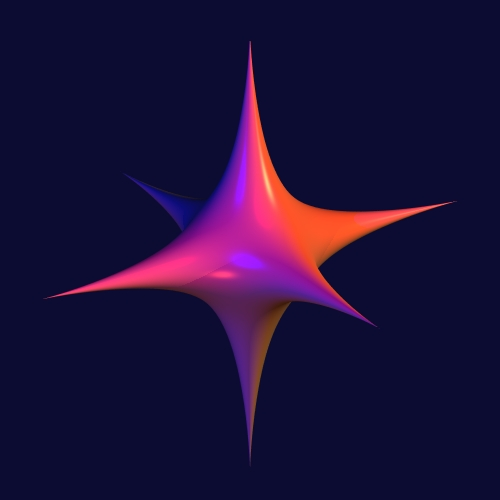
\includegraphics[scale=0.8]{./stern.jpeg}
\caption{Variety defined by the equation $x^2y^2 + y^2z^2 + x^2z^2 + 100 ( x^2 + y^2 + z^2 - 1)^
3 = 0$}
\label{fig:joe2}
\end{figure}

\end{textblock}

% References: -------------------------------------------------------

\begin{textblock}{8}[1,1](17,24.7)
    \small 
    

\bibliography{/home/jtait/Desktop/Work/Bibliography/biblio.bib}
\bibliographystyle{plain}

\end{textblock}






% --------------------------------------------------------------------

\end{document}

